\documentclass{beamer-control}
\usepackage{beamer-control-singlefile}
\INCLUDEONLY{Zero Frequency Gain, Poles, and Zeros}
\begin{document}
\CONCEPT{Zero Frequency Gain, Poles, and Zeros}

\begin{SUMMARY}
\begin{itemize}
\item Zero Frequency Gain
\item Poles and Zeros
\item Pole/Zero Cancellation
\end{itemize}
\vfill References:
\begin{itemize}
\item \astrom{Chapter Z}
\end{itemize}
\end{SUMMARY}



\SUBCONCEPT{Zero Frequency Gain}

\begin{frame}
Zero frequency gain (aka \alert{DC gain}) = magnitude of a transfer function at $s=0$:
\begin{align}
G(0) &= D - CA\Inv B
\end{align}
For a transfer function
\begin{align}
G(s) = \frac{b_0 s^m + b_1 s^{m-1} + \cdots + b_m}{s^n + a_1 s^{n-1} + \dots + a_n}
\end{align}
and therefore
\begin{align}
G(0) = \frac{b_m}{a_n}
\end{align}
From the final value theorem, $G(0)$ is the step response final value.
\end{frame}


\SUBCONCEPT{Poles and Zeros}

\begin{frame}{Poles}
For TF $G(s) = b(s)/a(s)$ with polynomials $b(s)$ and $a(s)$:
\begin{itemize}
\item Roots of $a(s)$ are \alert{poles}
\item Roots of $a(s)$ are the eigenvalues of $A$ \\(soln of $\det(sI-A)=0$)
\item A pole corresponds to a mode of the system with modal solution $\Exp{pt}$
\item Unforced motion of a system is a weighted sum of modes
\end{itemize}
\end{frame}

\begin{frame}{Zeros}
For TF $G(s) = b(s)/a(s)$ with polynomials $b(s)$ and $a(s)$:
\begin{itemize}
\item Roots of $b(s)$ are \alert{zeros}
\item A zero corresponds to a signal $\Exp{qt}$ which results in zero output (`blocked transmission')
\item For $n$ poles and $m$ zeros, $n_{pe} = n-m$ is the \alert{pole excess} or \alert{relative degree} of the TF
\item $n_{pe}\ge 0$ is a \alert{proper} system; $n_{pe}>0$ is \alert{strictly proper}
\item Zeros given by solutions of:
\end{itemize}
\begin{align}
\det\left(\Matr{sI-A & B\\C & D}\right)=0
\end{align}
\end{frame}

\begin{frame}
\frametitle{High Frequency Gain}
\begin{columns}
\column{0.33\textwidth}
\centerline{\textbf{Strictly proper}}

\column{0.33\textwidth}
\centerline{\textbf{Proper}}

\column{0.33\textwidth}
\centerline{\textbf{Improper}}
\end{columns}

\vspace*{0pt plus 1filll}
\null
\end{frame}

\begin{frame}
\frametitle{Pole zero map}

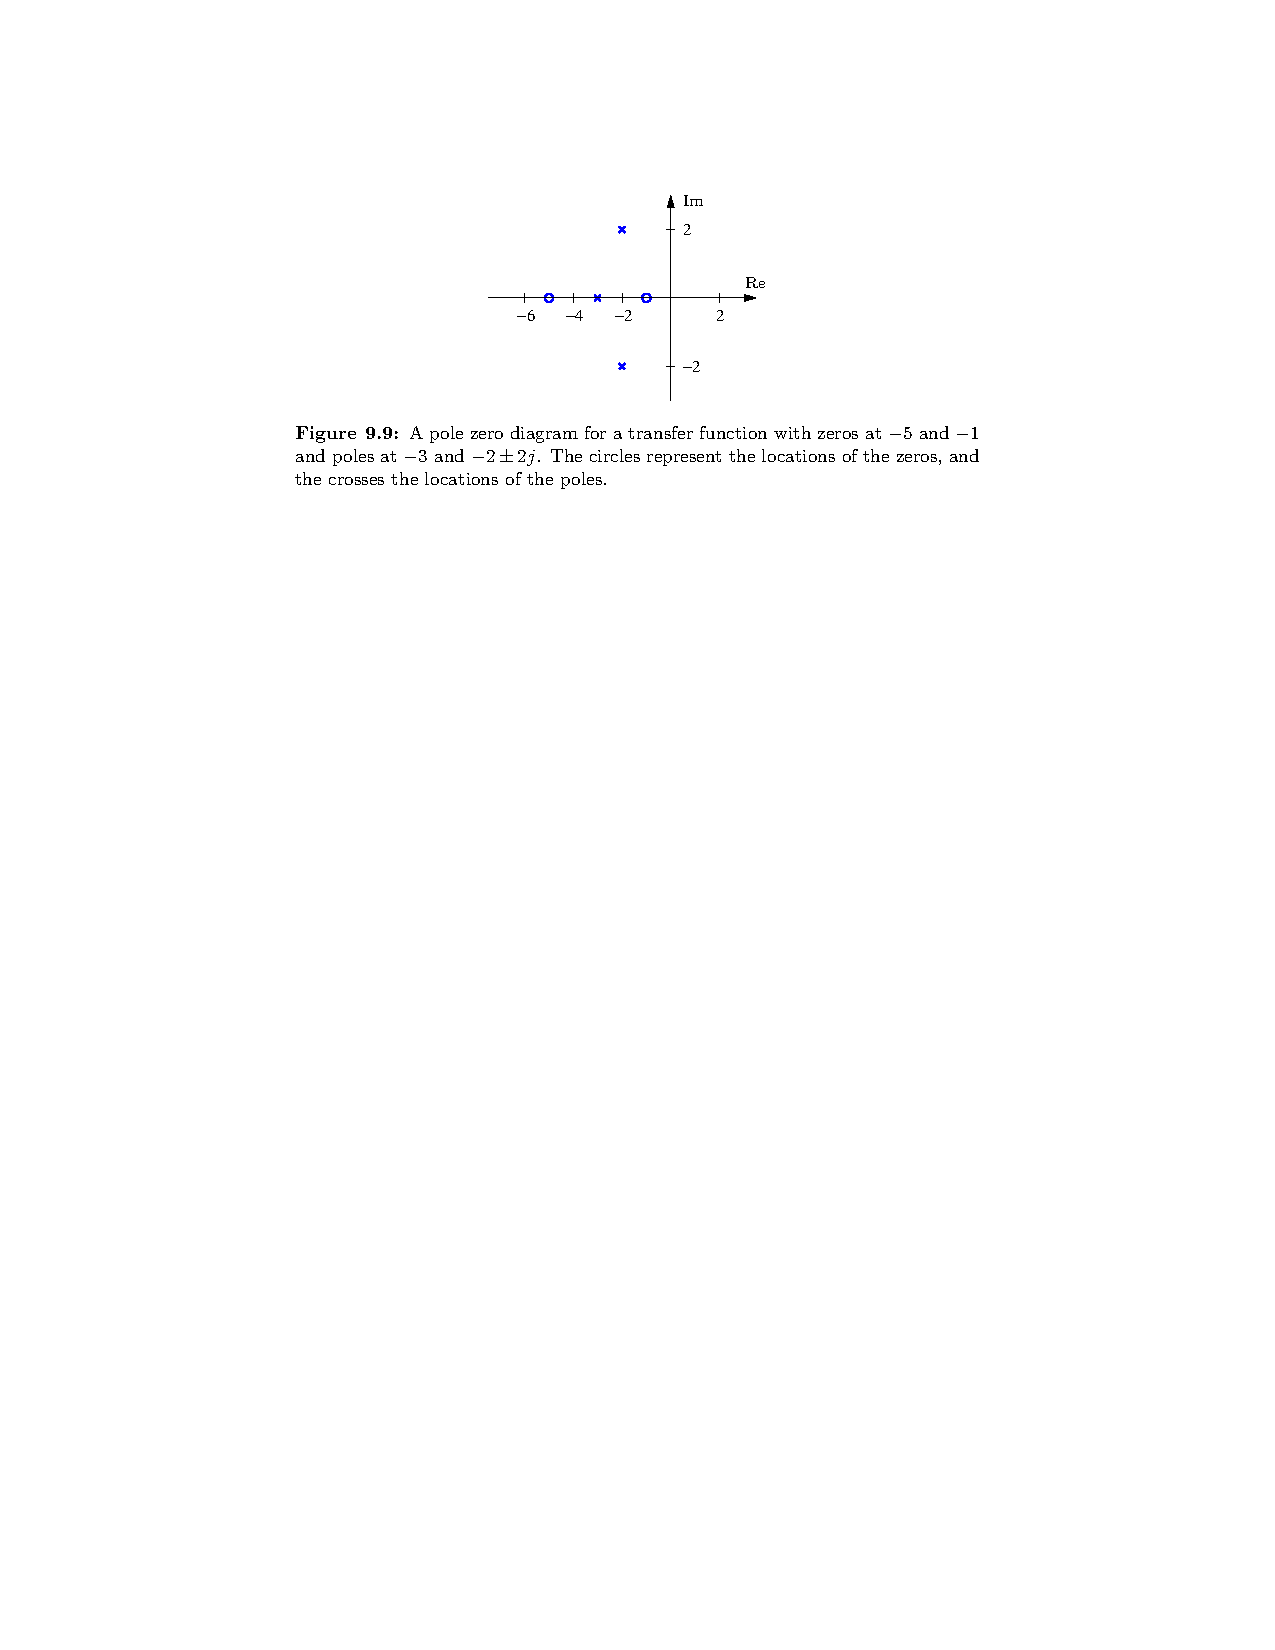
\includegraphics[width=\linewidth]{figure9.9}


\end{frame}

\SUBCONCEPT{Pole/Zero Cancellation}

\begin{frame}
\frametitle{}
\begin{itemize}
\item Sometimes poles and zeros end up with the same numerical value in a closed loop transfer function
\item Although they are `just' factors of polynomial equations, we have to be careful about cancelling them out (or not)
\end{itemize}
\begin{uncoverenv}<2->
Consider:
\begin{align}
P(s) &= \frac{s-1}{s^2+6s+s} & C(s) &= \frac{s+1}{(s-1)(s+2)}
\end{align}
\end{uncoverenv}

\begin{uncoverenv}<3->
In this case, with pole-zero cancellation we have:
\begin{align}
CP &= \frac{s-1}{(s+1)(s+5)}\cdot\frac{s+1}{(s-1)(s+2)}=\frac{s+1}{(s+1)(s+2)(s+5)}
\end{align}
which is a `stable' TF and will have stable closed loop dynamics. But\dots
\end{uncoverenv}
\end{frame}

\begin{frame}
\frametitle{Robustness}
\begin{itemize}
\item
Can't have an unstable controller (!)
\item
What if the pole and zero approach the same value but are not exactly equal?
\item
What about other paths through the block diagram?
\end{itemize}
\centerline{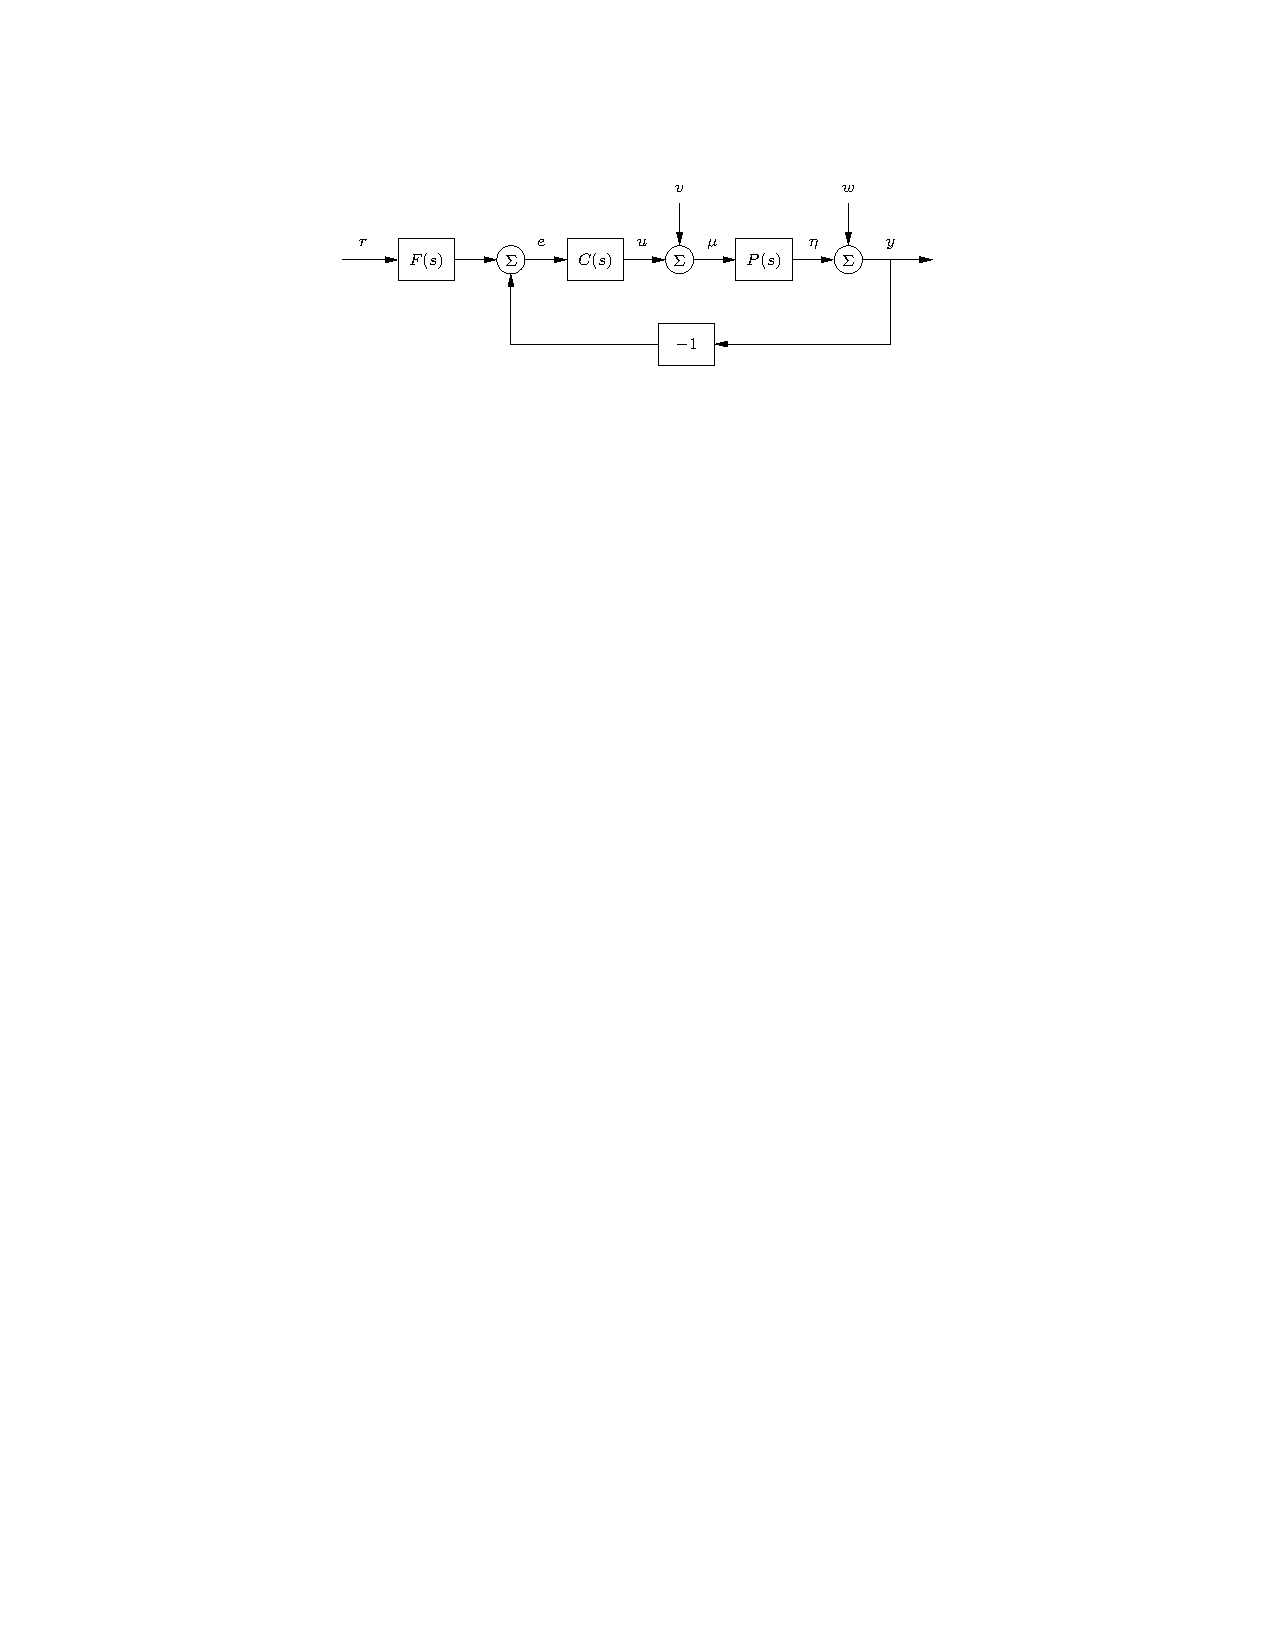
\includegraphics[width=0.7\linewidth]{figure9.6}}
\begin{align}
G_{yr} &= \frac{CP}{1+CP} &
G_{yv} &= \frac{P}{1+CP} &
G_{yw} &= \frac{1}{1+CP}
\end{align}
\end{frame}

\SUMMARYFRAME
\FINALE

\end{document}
